%% SW klassediagram static

\begin{figure}[!htbp] \centering
{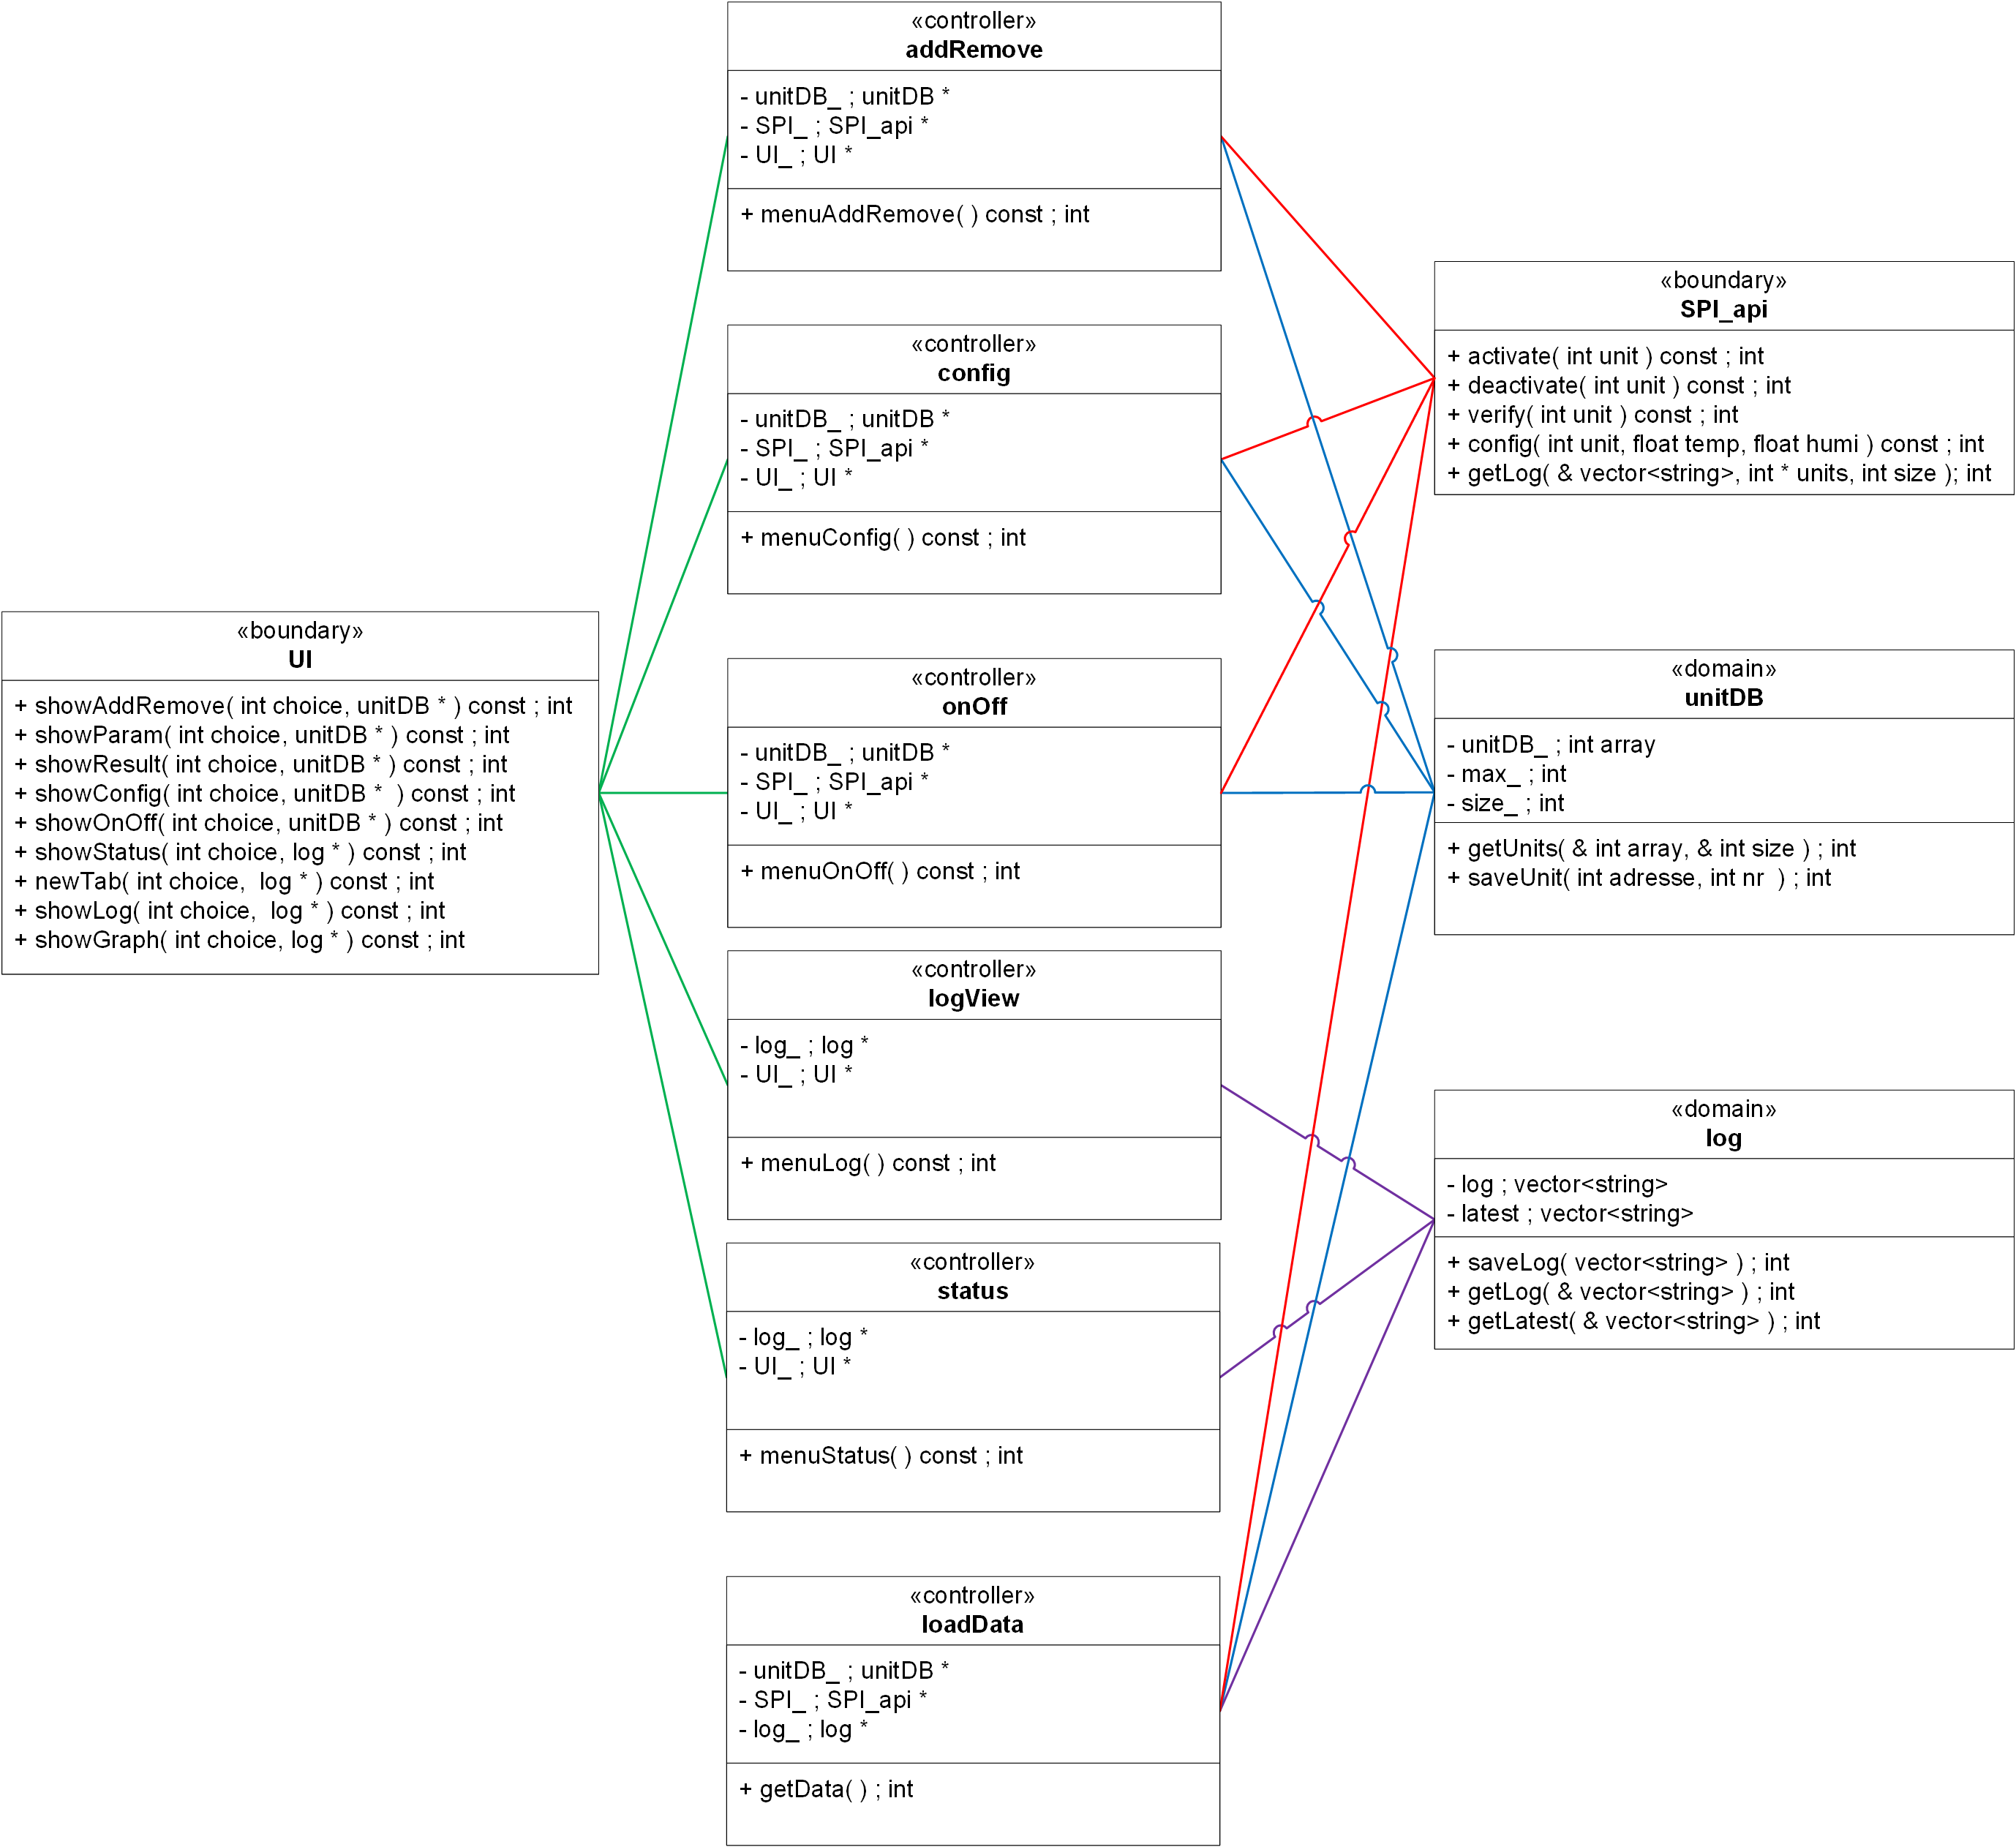
\includegraphics[scale=0.7]{filer/design/sw_class_devkit_static}}
\caption{Statisk klassediagram for Master (Devit8000)}
\label{fig:class_static_dev}
\end{figure}

Da Vi har arbejdet i Qt frameworket til at oprette og styre vores user interface på Devkit8000 så har vi gjort brug af mange af deres klasser. F.eks anvendes der ofte en QString istedet for en std::string. Der er design billeder der viser hvordan vores UI ser ud når det bliver deployed på devkittet. Design filerne er dem i UI klassen som starter med win som ses på figur \ref{fig:class_static_dev}. Disse UI billeder har nogle knapper som kan sende nogle signaler til vores funktioner, et såkaldt event system. Event systemet er det som bringer os rundt i UI'en ved at kalde nogle bestemte funktioner når de pågældende knapper bliver trykket på osv.
